\documentclass[12pt]{exam}
\newcommand{\hwnumber}{8}
\newcommand{\hwname}{Peg Solitaire}
\newcommand{\duedate}{\formatdate{31}{10}{\YEAR} by \progDueTime} % day-month-year

\usepackage{../misc/latex/edition}  % Course semester
\usepackage{../misc/latex/c0}       % Listings style for c0
\usepackage{amsmath}
\usepackage{enumerate}
\usepackage[normalem]{ulem}
\usepackage{verbatim}
\usepackage[left=1in, right=1in, top=1in, bottom=1in]{geometry}
\usepackage{graphicx}
\usepackage{hyperref}
\usepackage{tikz}     \usetikzlibrary{shapes}
\usepackage{fancybox}
\usepackage[all]{xy}
\usepackage{wrapfig}
\usepackage{fancyvrb}
\usepackage{datetime}
\usepackage{etoolbox}
\usepackage{calc}
\usepackage[nomessages]{fp}
\usepackage{import}  % Like input and include, but respects subdirectories

\newcommand{\defaultQuestionLocation}{questions}
\newcommand{\inputQuestion}[2][\defaultQuestionLocation/]{%
  \subimport{#1}{#2}
}
% Subdirectories of \defaultQuestionLocation containing code and pictures
\newcommand{\code}{code}
\newcommand{\img}{img}


%%% ic: frontmatter macros
\newcommand{\specialInstructions}{}
\newcommand{\HWNUMBER}
{\ifdefempty{\hwnumber}{__}{%
  \ifnumless{\hwnumber}{10}{0\hwnumber}{\hwnumber}}}
\newcommand{\hwtype}{Written Homework}

%%% ic: 'exam' tweaks
\renewcommand{\half}{.5} % Half points

\newcommand{\Question}[2][]
 {\ifstrempty{#1}
    {\question{\bf #2}}
    {\question[#1]{\bf #2}}
  \immediate\write\rubricfile{}%
  \immediate\write\rubricfile{Question \thequestiontitle:}%
  \immediate\write\rubricfile{==========}
 }

%%% ic: Support for editable PDF
% counter name (some viewers misbehave if always the same)
\newcounter{editable}
\newcommand{\nextField}{\addtocounter{editable}{1}q\arabic{editable}}
\newcommand{\NextField}
 {\makebox[0pt][r]{\scalebox{0.1}{\color{White}\nextField}}}

% Color of edit area
\newcommand{\editAreaColor}{red}
% Single line answer:   \editableLine[extra parameters (optional)]{line width}
\newcommand{\editableLine}[2][]
{\textcolor{\editAreaColor}{%
 \underline{\hspace*{-0.25em}%
 \raisebox{-0.5ex}{%
 \TextField[width=#2, borderwidth=0, #1]{\NextField}}}}%
}
% Single line answer for code:  \editableLine[extra parameters (optional)]{line width}
\newcommand{\editableCodeLine}[2][]
{\textcolor{\editAreaColor}{%
 \underline{%
 \TextField[width=#2, height=1.5ex, borderwidth=0, #1]{\NextField}}}}
% Multiline answer:  \editableLine[extra parameters (optional)]{box height}
\newcommand{\editableBox}[2][]
{\leavevmode\hspace*{-0.1em}%
\TextField[height=#2, width=\linewidth,
           multiline=true, borderwidth=0.1, bordercolor=\editAreaColor,
           #1]{\NextField}}

%%%%% Same answer format as exams
\renewcommand{\rmdefault}{ppl}
\renewcommand{\sfdefault}{phv}
\newcommand{\answerColor}{Blue}

\ifprintanswers
\newcommand{\answer}[2]{\makebox[#1][c]{\color{\answerColor}#2}}
\else
\newcommand{\answer}[2]{\makebox[#1][c]{}\makebox[0pt]{\phantom{|}}}
\fi
\newcommand{\uanswer}[2]{\underline{\answer{#1}{#2}}}


%%% Write rubric snippet.  Usage:
% \RUBRIC
% any multi-line text (including \, #, %, whatever)
% ENDRUBRIC
%% (ENDRUBRIC should be on a line by itself)
\makeatletter
\def\RUBRIC
 {%
  \begingroup
  \let\do\@makeother\dospecials
  \endlinechar=`\^^J
  \@tofile%
 }
\def\ENDRUBRIC{ENDRUBRIC}
\def\@tofile#1^^J{%
  \def\@test{#1}%
  \ifx\@test\ENDRUBRIC
    \immediate\write\rubricfile{}  % End with an empty line
    \expandafter\@firstoftwo
  \else
    \expandafter\@secondoftwo
  \fi
  {\endgroup}%
  {\toks@{#1}%
   \begingroup\endlinechar=\m@ne
   \everyeof{\noexpand}%
   \xdef\@temp{\scantokens\expandafter{\the\toks@}}%
   \endgroup
   \immediate\write\rubricfile{\@temp}%
   \@tofile}%
}
\makeatother

%% Displays tags for an exercise in 'answer' mode
\newcommand{\TAGS}[1]
{\ifprintanswers%
  \rule{0em}{0ex}%
  \marginpar{\footnotesize%
    \fcolorbox{black}{Gray!25}{%
      \parbox[t]{2cm}{\raggedright\textbf{TAGS:}\\#1}}}%
  \ignorespaces%
 \fi}%


%% Page layout
\pagestyle{headandfoot}

\headrule
\header{\textbf{\courseNumber{} \hwtype{} \hwnumber}}
       {}
       {\textbf{Page \thepage\ of \numpages}}
\footrule
\footer{}{}{\COPYRIGHT}

\renewcommand{\partlabel}{\textbf{\thequestion.\thepartno}}
%\renewcommand{\partlabel}{\textbf{Task \thepartno}}
\renewcommand{\subpartlabel}{\textbf{\thesubpart.}}
\renewcommand{\thepartno}{\arabic{partno}}
\renewcommand{\thesubpart}{\alph{subpart}}
\pointpoints{pt}{pts}
\pointformat{\raisebox{0ex}[\height][0pt]{\fcolorbox{black}{yellow}{\themarginpoints}}}
\bonuspointformat{\raisebox{0ex}[\height][0pt]{\fcolorbox{black}{red}{\themarginpoints}}}
\marginpointname{\points}
\pointsinmargin
%\boxedpoints

\setlength\answerlinelength{2in}
\setlength\answerskip{0.3in}

\newcommand{\mkWrittenTitle}[1]{#1}
\newcommand{\mkDueDate}[1]{#1}
\newcommand{\mkEvalSummary}[1]{#1}
\newcommand{\mkGradetable}[1]{#1}



% This fixes an issue with the exam package version 2.6 and after,
% where 'framed' has been renamed to 'examframed' to avoid a conflict.
\ifcsmacro{examframed}{%
\newenvironment{framed}
{\begin{examframed}}
{\end{examframed}}
}{}

\begin{document}
\hwTitle

\noindent
For the programming portion of this week's homework, you will
implement a program to solve peg solitaire puzzles.


\bigskip
\noindent
The code handout for this assignment is at
\begin{center}
\whereisthetgz{peg-handout.tgz}
\end{center}
The file \lstinline'README.txt' in the code handout goes over the
contents of the handout and explains how to hand the assignment in.
There is a FIFTEEN (15) PENALTY-FREE HANDIN LIMIT.  Every additional
handin will incur a small (5\%) penalty (even if
using a late day).


\paragraph{Modification to the academic integrity and \qatoolName{} policy}

For this assignment, it is permissible (and encouraged!) to share game
boards (test input), as long as you do this sharing publicly on
\qatool{}.  Tag these \qatoolName{} posts by writing
\lstinline'#needaboard' in the post.

\paragraph{Style and contract testing}

This assignment will \textbf{not} be graded for style.  However you
will still find it helpful to employ good style habits: reasonable
contracts, at most 80-character lines, and comments that make it clear
to a reader how your algorithm works and what invariants you expect to
hold. You should use the libraries provided for you to make your code
simpler and clearer. We expect you to write your own helper functions
when appropriate.  Bad style will have no direct effect on your grade
but will make your life harder.

One reason for this is that your code is liable to get pretty messy as
you transform your code to make it more efficient. In order to succeed
at this assignment, you will want to \emph{refactor} your code ---
notice that it has gotten complicated and restructure it in a way that
suits the task better. Refactoring a bit will help you write and debug
the assignments.


\newpage
\section*{Peg Solitaire}
\label{sec:peg}

\emph{Peg solitaire} is a one-player board game with the goal of
removing all pegs except one from a board, starting with some initial
board configuration consisting of holes, some of which are filled with
pegs.

A move is always a vertical or horizontal jump of one peg over another
into a hole, removing the peg that was jumped over from the board.
For example, in the initial configuration of the \emph{standard
  English board} on the left, there are 4 possible moves
(highlighted), all ending with a peg in the center hole.  The peg
arriving from the top leads to the configuration on the right, where
we have now have just 3 possible moves (also highlighted).
\begin{center}
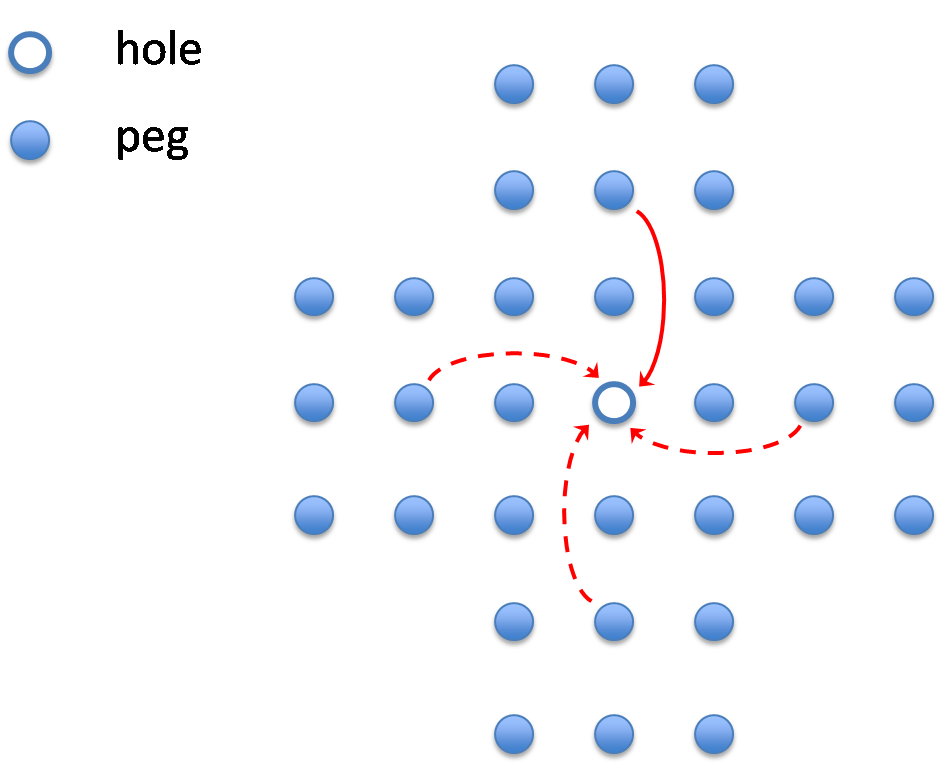
\includegraphics[width=0.4\textwidth]{\img/peg1.png}
\hspace{3em}
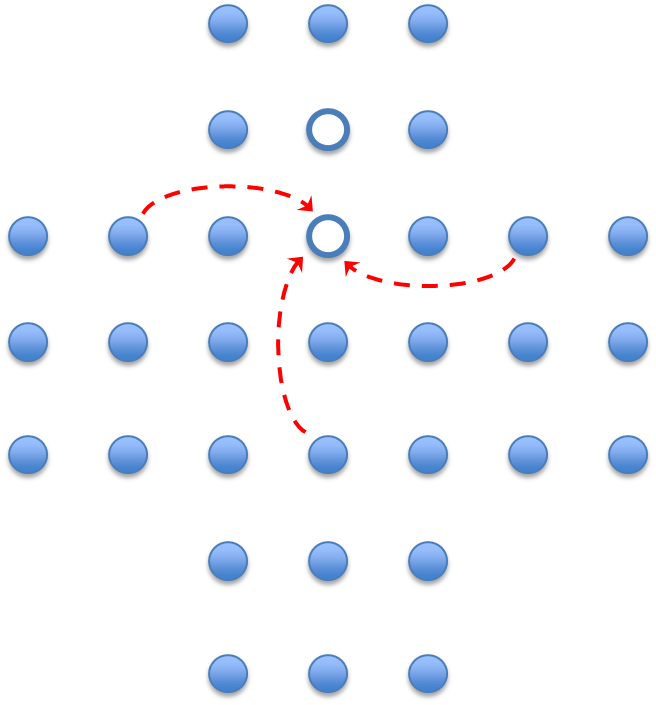
\includegraphics[width=0.28\textwidth]{\img/peg2.png}
\end{center}

The goal of the game is to be left with just one peg. On the standard
English board we start with 32 pegs, so any solution will require
exactly 31 moves (each jump removes one peg from the board).  In some
variations of the game we also stipulate where the final peg should
come to rest, but in this assignment reaching a board with a single
peg is the only goal.  See
\url{http://en.wikipedia.org/wiki/Peg_solitaire} for more on peg
solitaire.


\enlargethispage{5ex}
\subsubsection*{Games computers play}

The structure of peg solitaire is well suited to a solution involving
recursion.  If we want to play peg solitaire on a board with 32 pegs,
we can enumerate all the valid moves that can be made on that
board. Then, after we make one of those moves, we're playing peg
solitaire again --- only this time on a board with 31 pegs.
\begin{center}
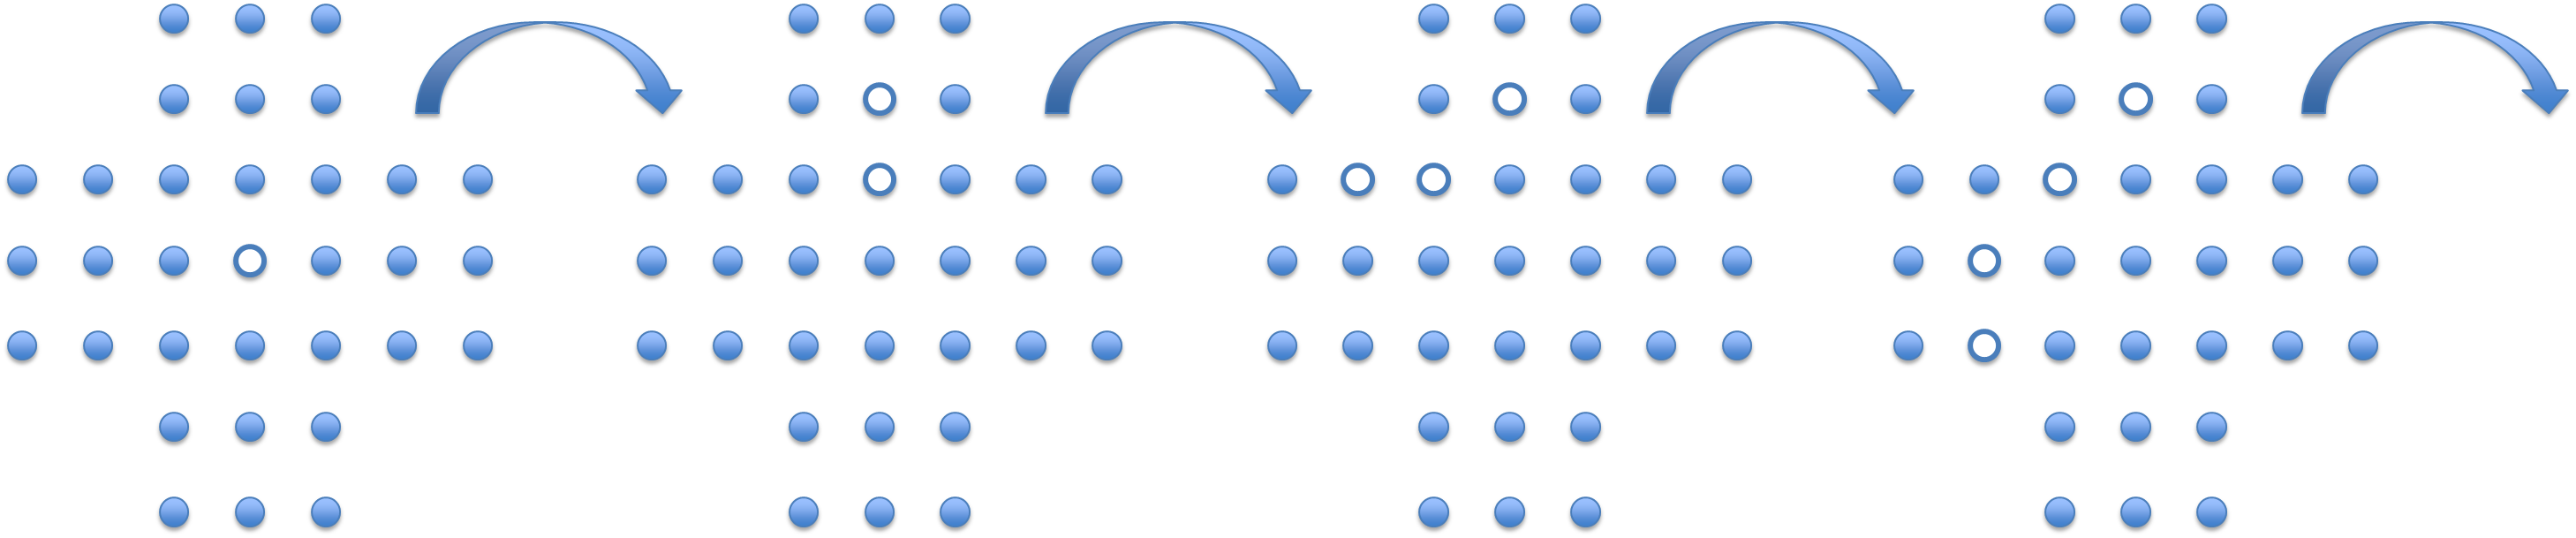
\includegraphics[width=\textwidth]{\img/pegpath1.png}
\end{center}
If we ever reach a point where we're playing peg solitaire on a board
with one peg, we've won! A \emph{losing} game
of peg solitaire is one where there are no valid moves and more than
one peg. An \emph{unsolvable} game of peg solitaire is one where every
series of valid moves leads to a losing game.


\newpage
\section{Game Representation}

When writing a program that plays a game, there are two distinct
phases: representing the the game itself (boards, moves, etc), and
solving the game (finding a solution or determining it is unsolvable).
We now consider representing the game.  We will fix the representation
of boards and solutions for you, but let you decide how to represent
moves.


\subsection{Representing the Board}

Abstractly, we think of a peg solitaire board as an $8 \times 8$ grid
of pegs, holes and blocked locations.  Here is an abstract view of the
standard English board:
\begin{center}
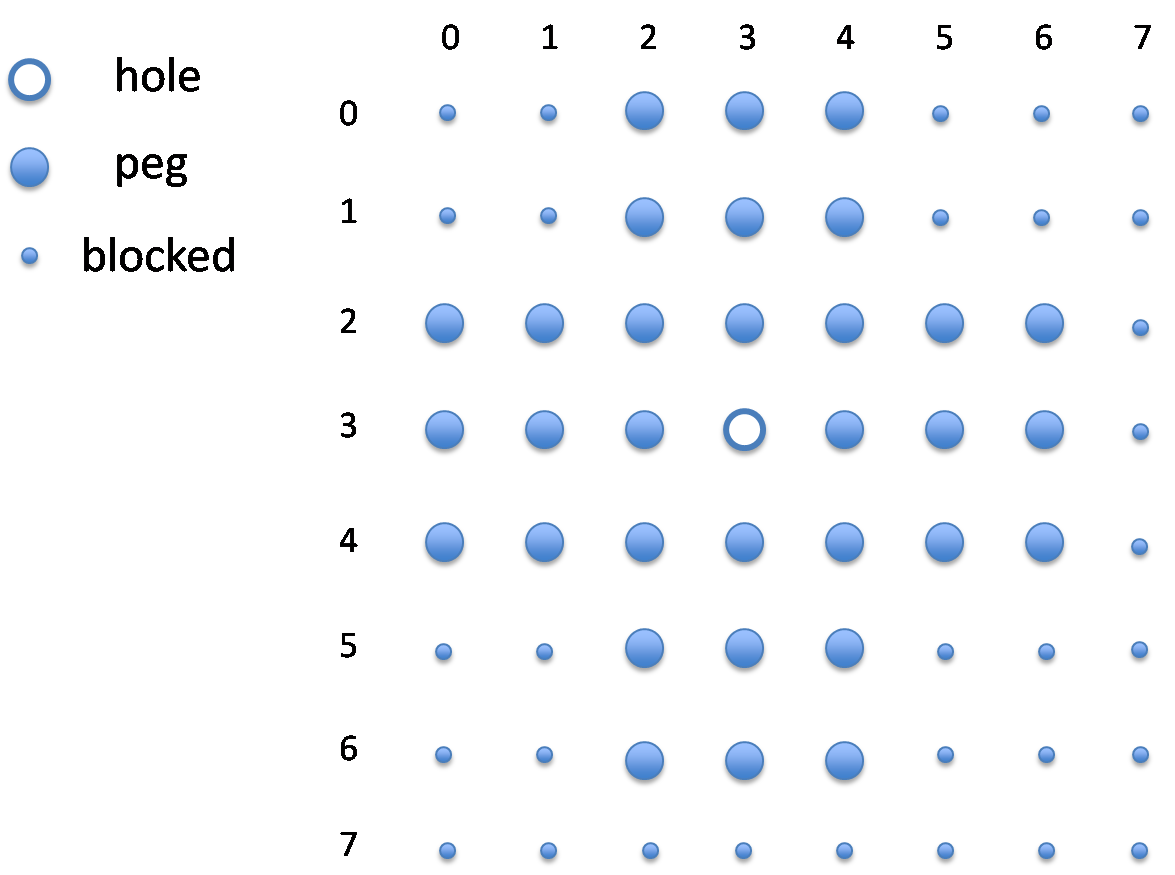
\includegraphics[width=0.6\textwidth]{\img/peg3.png}
\end{center}
Other boards have different configurations of pegs, holes and blocked
locations, but they will always fit into an $8 \times 8$ grid.  The
notation we use for a location on a board is $\mathit{row} {:}
\mathit{col}$, starting both $\mathit{row}$ and $\mathit{col}$ at 0 in
the upper left-hand corner.  For example, the one hole in this board
is at location \lstinline'3:3', the peg we used for our example move
on the previous page is at location \lstinline'1:3', and the blocked
location at the top-right corner is \lstinline'0:7'.

In this programming assignment, we \emph{concretely} represent a peg
solitaire board as an array of $8 \times 8 = 64$ integers.  The value
$-1$ means the location is blocked, $0$ means the location is a hole
without a peg, and $1$ means the location is a hole occupied by a peg.
A valid board cannot contain other values.  We represent a board by
concatenating its rows as a one-dimensional array.  Thus, location
\lstinline'1:3' corresponds to array index $1*8+3 = 11$ in the board
array, \lstinline'3:3' corresponds to array index $3*8+3 = 27$, and
\lstinline'0:7' corresponds to index $0*8+7 = 7$.  Please refer to the
definitions in the file \lstinline'lib/peg-util.c1', including
\begin{lstlisting}
typedef int[] board;
\end{lstlisting}
This file also contains functions to read board configurations from a
file and print board configurations.


\subsection{Representing a Move}

It is up to you how to represent moves, but we expect the type
\lstinline'move' to be a pointer type:
\newcommand{\hwstar}{\commentstyle{*}}
\begin{lstlisting}
// typedef ________[*\hwstar{}*] move;
\end{lstlisting}
Some suggestions for representations: triples of integers
(representing the three board indices involved), pairs of integers
(the first and last array index of the move), or four integers
representing the row and column values of the peg before and after the
move.  These could be represented by structs, or could be compressed
into something like a single \lstinline'int'.  This involves a
trade-off between compactness and ease or speed of determining the
possible moves on a given board --- this may be important later when
solving the game.  Note that we do \textbf{not} combine multiple jumps
into a single move.

\begin{task}[3]
\TAGS{correctness, ds-invariant, safety}
In file \lstinline'peg-moves.c1', define the type \lstinline'move'
\begin{lstlisting}
// typedef ________[*\hwstar{}*] move;
\end{lstlisting}
and implement the following five functions:
\begin{lstlisting}
move new_move(int from_row, int from_col, int to_row, int to_col);
int row_start(move m);
int col_start(move m);
int row_end(move m);
int col_end(move m);
\end{lstlisting}
They create a new move based on the starting and ending locations of
the jumping peg, and extract the row and column of these locations
from your representation of a move.  You should include contracts that
catch invalid locations or jumps.  We strongly suggest that you write
contracts that validate moves.
\end{task}

The testing harness will treat the type \lstinline'move' as abstract.
This means it only uses these five functions to create and inspect a
move.  You can find the testing harness in
\lstinline'peg-main.c1'. You cannot change this file, but you can
inspect this code (and the code in \lstinline'lib/peg-util.c1') and
reuse anything you find useful.

\bigskip

We play peg solitaire by making moves.  Your next task will be to
implement a function that makes a (single) move on a given board.  It
will later be useful to also be able to \emph{undo} a move.

\begin{task}[2]
\TAGS{correctness, ds-invariant, safety}
Implement the functions
\begin{lstlisting}
void make_move(board B, move m);
void undo_move(board B, move m);
\end{lstlisting}
For \lstinline'make_move', a contract should fail if the move is
invalid according to the rules of peg solitaire.  Similarly,
\lstinline'undo_move(B, m)' should fail a contract if board
\lstinline'B' could not have been reached by making move \lstinline'm'
from any valid board.  This means you will need to write strong
representation invariants for moves and boards.
\end{task}

\bigskip

In order to play peg solitaire, we will need to find all the valid
moves that can be played on a given board.  In the case of the
standard English board on page~\pageref{sec:peg}, that would be the
four moves highlighted in the top-left figure.

\begin{task}[3]
\TAGS{genericity, stack, void-star}
Implement the function
\begin{lstlisting}
void all_moves(board B, stack_t M);
\end{lstlisting}
that stores all the valid (one-step) moves for board \lstinline'B' into
the stack \lstinline'M' (in any order but without repetitions).  The
file \lstinline'lib/stacks.c1' provides an implementation of
\emph{generic} stacks.
\end{task}


\subsection{Representing a Solution}

A \emph{solution} to peg solitaire from a given initial board
consists of a \emph{stack of moves}.  The top of the stack should
contain the first move, the next element the second move, etc.  The
function
\begin{lstlisting}
bool verify_solution(board B, stack_t Sol);
\end{lstlisting}
(provided in file \lstinline'peg-main.c1') verifies that the stack
\lstinline'Sol' is a valid solution for the initial configuration
given by board \lstinline'B'.


\section{Solving Peg Solitaire}

Now that we have a representation for peg solitaire and related
concepts, we will solve it, i.e., determine whether a given board is
solvable, and if so return a solution.  We will do so in two steps.
We will first write a solver that works well for boards with just a
few pegs but that is too slow for most larger boards.  We will then
refine this solver to work for many more boards (although it too may
time out for really complicated boards).


\subsection{A Simple Solver}

To solve a puzzle like peg solitaire, we pick a valid move, apply it
to the current board, pick a valid move from that board, apply it, and
so on until we get to a winning board.  Since each move removes one
peg, we will be done after a specific number of moves (31 in the case
of the standard English board, which starts with 32 pegs) \ldots~if we
are lucky.

But what if we pick a wrong move and end up on a losing board?  Here's
an example where we tried \lstinline'1:2' to \lstinline'1:0' as our
first move and \lstinline'2:1' to \lstinline'2:3' as our second move
(only locations with a hole or a peg are shown, and only attempted
moves are highlighted):
\begin{center}
  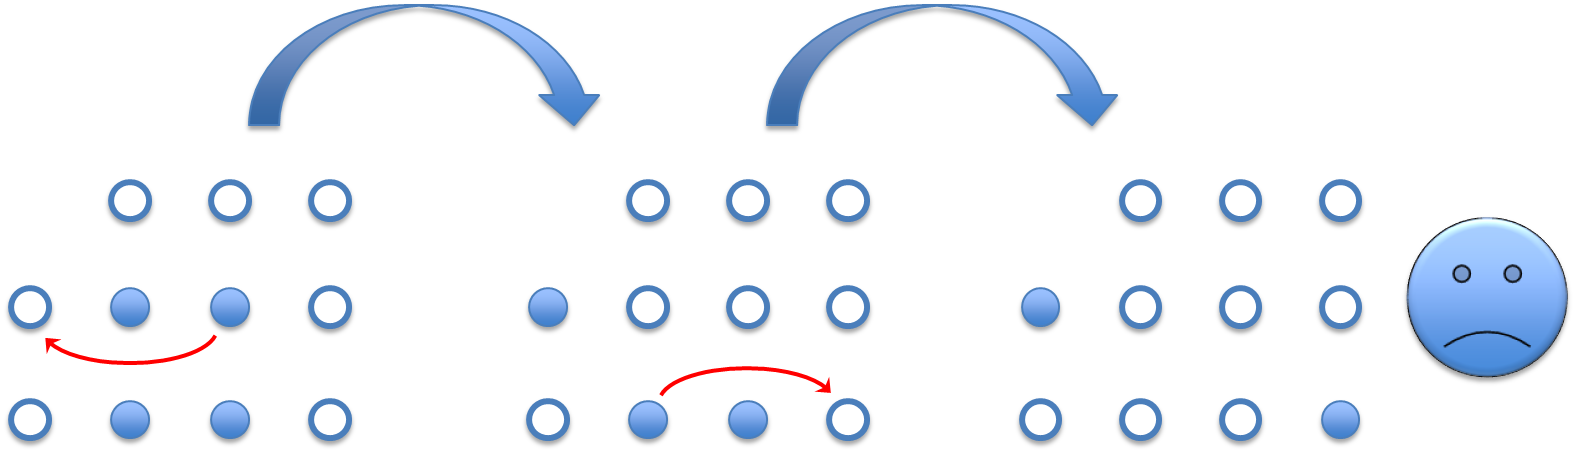
\includegraphics[width=0.7\textwidth]{\img/pegpath2.png}
\end{center}
This didn't work.  We need to go back and consider a different move, a
strategy called \emph{backtracking}.  Right now we know that the third
peg solitaire board above, with two pegs, is a losing game, which
means it is unsolvable.  But we don't know that the \emph{second} peg
solitaire board, the one with three pegs, is unsolvable, because
there's another valid move we could make --- \lstinline'2:2' to
\lstinline'2:0'. So we backtrack to this old board and try this
alternative move:
\begin{center}
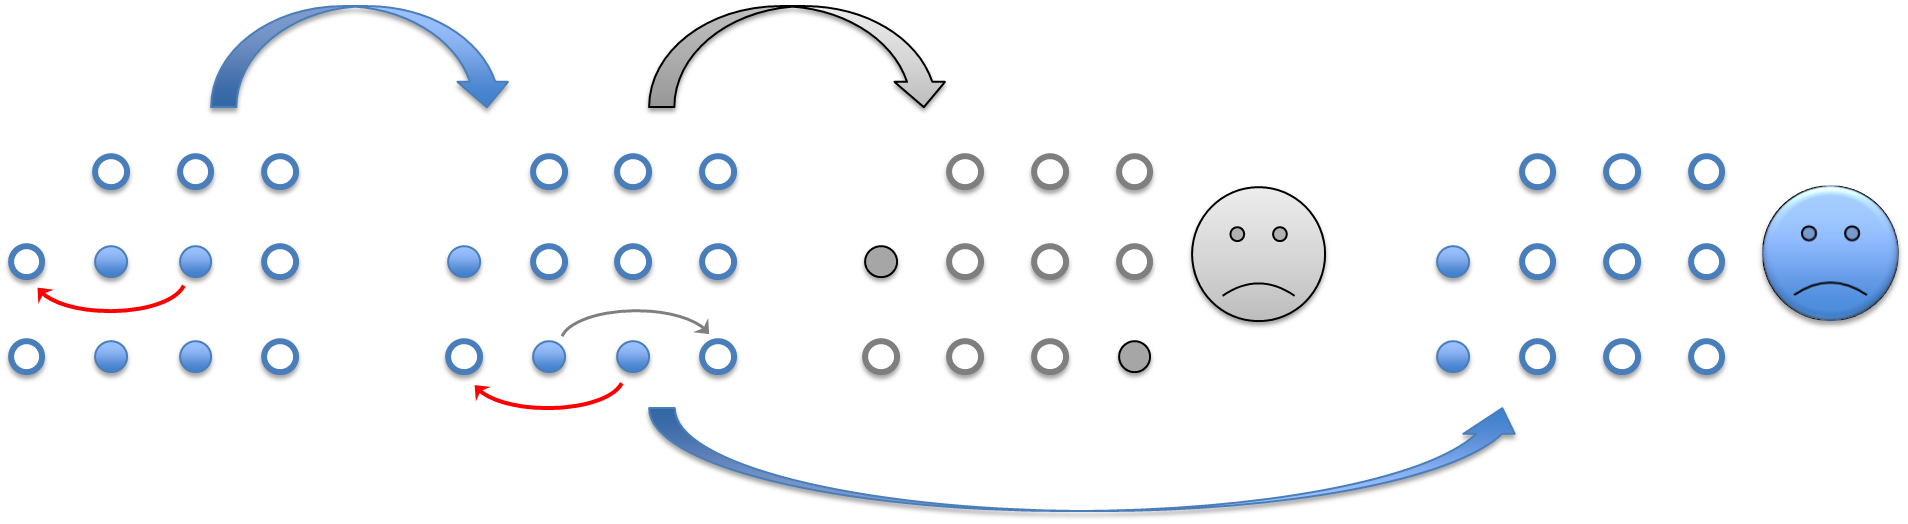
\includegraphics[width=\textwidth]{\img/pegpath3.png}
\end{center}
Unfortunately, this second move also leads to a losing board. This
means that the board with three pegs above \emph{is} unsolvable ---
all the moves starting from that board lead to losing boards.  We have
to backtrack further, to the board with four pegs, and pick a
different way forward. If we pick the valid move \lstinline'2:1' to
\lstinline'0:1', we will succeed:
\begin{center}
\hspace*{-4em}%
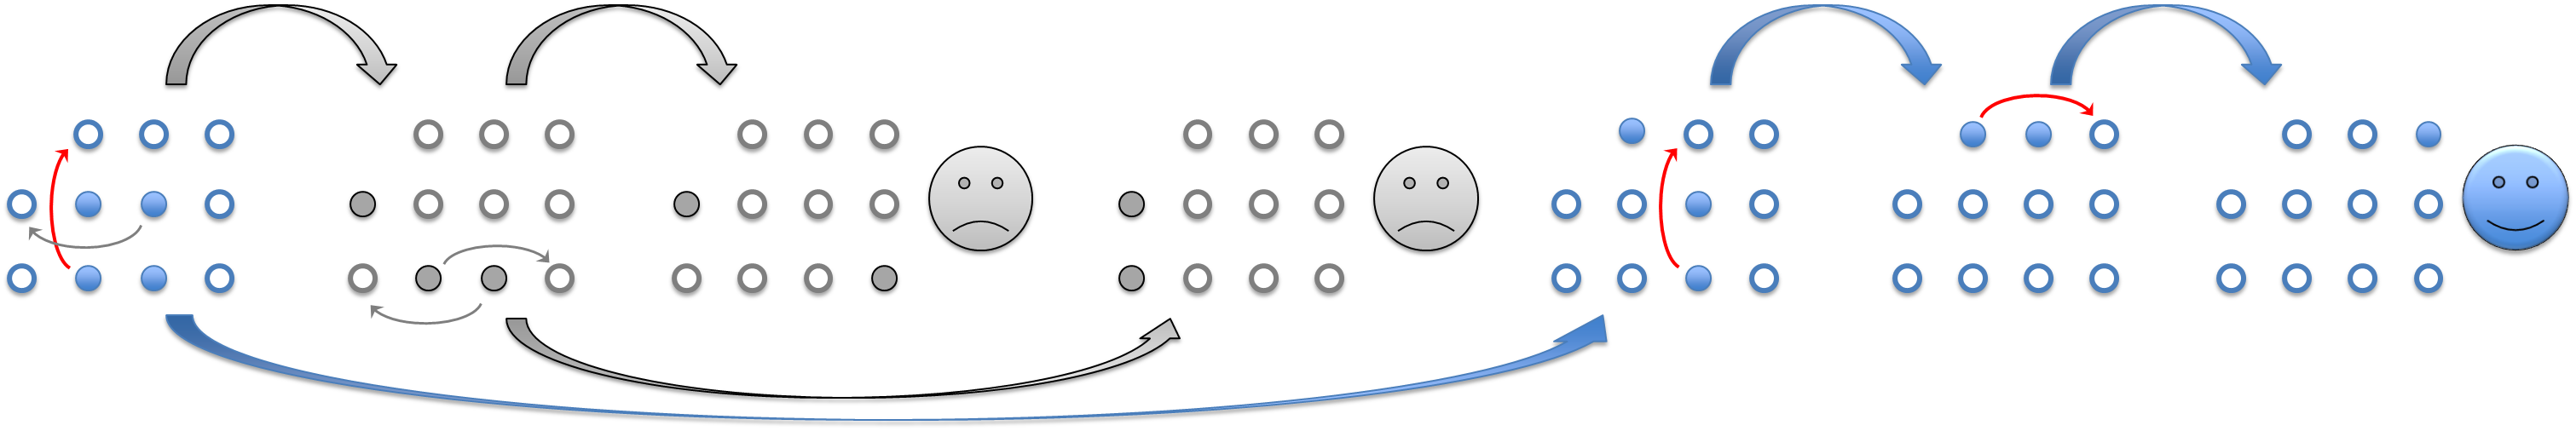
\includegraphics[width=1.2\textwidth]{\img/pegpath4.png}
\end{center}
To summarize, when we hits a dead-end with no moves left to try, we
undo the previous move and try another move.  It that fails, we
undo that move and repeat this process.

\medskip

You will now write a backtracking solver for peg solitaire.  At each
step, you will compute all valid moves, pick one of them while
remembering the others, make that move and repeat until you either
stumble upon a board with a single peg or onto one with several pegs
left but no possible moves.  In the first case, you shall report that
the initial board was solvable and return the sequence of moves that
led to a solution.  In the second case, you will need to go back and
try another move.

\begin{task}[8]
\TAGS{ds-traversal, search}
In the file \lstinline'peg1.c1', implement the function
\begin{lstlisting}
int solve(board B, stack_t Sol);
\end{lstlisting}
to search for a solution to peg solitaire for board \lstinline'B'.
The integer that \lstinline'solve' returns is the smallest number of
pegs that playing the game starting from \lstinline'B' can end with.
Therefore,
\begin{itemize}
\item%
  if \lstinline'solve' returns \lstinline'1', then your algorithm
  played peg solitaire and won.  In this case, \lstinline'Sol' should
  contain a solution in the form of a stack of moves.
\item%
  if \lstinline'solve' returns a number greater than \lstinline'1',
  then your algorithm tried all possible sequences of moves from board
  \lstinline'B' and the best it could achieve was to remove all but
  \lstinline'\result' pegs.  In this case, \lstinline'Sol' can contain
  anything.
\end{itemize}
\end{task}

While you are welcome to implement your solver any way you want, a
recursive implementation is particularly straightforward as it frees
you from having to explicitly manage backtracking.  If you use
recursion, you will want to write a \emph{recursive} helper function
\lstinline'solve_peg' that is called from \lstinline'solve'.  This
helper function could take the board, the current stack of moves, and
the number of pegs remaining on the board as parameters.  It should
return \lstinline"1" if there is a solution for the given
parameters. It should also alter the given solution stack by adding
the moves for the solution.  Questions you will need to think about:
\emph{What is the base case for this recursive function?}
\emph{When do you know you have a solution for the current board?}

% 0. If this is a winning board, return reporting it

% 1. Find all moves

% 2. If there are no moves, report the number of pegs.

% 3. As long as there still are moves to try

% 4(a). Pick a move and apply it

% 4(b). Search for a solution from the resulting board (with one fewer pegs)

% 4(c). If a solution was found, extend it with the picked move and return
% reporting this was a winning board

% 5. If all moves have been tried, report the minimum number of pegs you
% could get down to.


\subsubsection*{Testing}

You can test your solution by compiling it as described in
\lstinline'README.txt' and then running
\begin{lstlisting}[language={[coin]C}]
% ./peg1 german.txt
\end{lstlisting}
This one trivial test won't tell you very much, however.  You can then
move to small unit tests and easy-to-solve boards with the
\lstinline'-d' option as described in \lstinline'README.txt'.
\par\medskip\noindent
\bgroup\bf\small
\texttt{\%}~\lstinline[language={[coin]C}]'cc0 -d -o peg1 lib/peg-util.c1 lib/stacks.c1 peg1.c1 peg-main.c1'\\
\texttt{\%}~\lstinline[language={[coin]C}]'./peg1 medium_board_of_your_choice.txt'
\egroup
\par\medskip\noindent
Then, by compiling with the ``fast but unsafe'' options described in
the \lstinline'README.txt', you should try solving some trickier boards.
\par\medskip\noindent
\bgroup\bf\small
\texttt{\%}~\lstinline[language={[coin]C}]'cc0 -o peg1 -r unsafe -c-O2 lib/peg-util.c1 lib/stacks.c1 peg1.c1 peg-main.c1'\\
\texttt{\%}~\lstinline[language={[coin]C}]'./peg1 english.txt'
\egroup
\par\medskip\noindent
We will test your code using boards of increasing difficulty,
culminating in \lstinline'english.txt', the standard English board.
Depending on the order in which you pick moves, your code may or may
not be able to handle \lstinline'english.txt': we will run your solver
on it but not count it against your grade for this task.

We will set timeouts on the Autolab server so that if your code is too
slow it may fail some of the more difficult tests.  So you should pay
attention to the efficiency of your code.  You should be aware that
the Autolab server may run slower than your laptop (for instance).


\subsubsection*{Some Advice}

Your solver will need to be efficient.  Here are some thoughts:
\begin{itemize}
\item%
  Since applying a move modifies the board, after backtracking you
  must attempt the next alternative move on the original board.  If
  you make a copy of the board before attempting each move, your code
  will probably be too slow.  Instead, you may consider \emph{undoing}
  the change to the board when backtracking (this yields a useful
  invariant for the \lstinline'solve_peg' function: before it returns
  the board must be restored to the configuration it was in when it
  was called).
\item%
  You should have an efficient way to check that you have reached a
  winning configuration since you may have to do this many times.
\item%
  Almost any definition for the type \lstinline'move' in
  \lstinline'peg-moves.c1' will be good enough to get full
  credit.  However, depending on how the rest of your code is designed,
  you may notice an efficiency improvement if you represent moves
  as single integer.  Whether to do this is entirely up to you.
\end{itemize}
Said this, we ask you \emph{not to use hash tables} to speed up your
code.  This will allow you to explore how complex the problem can be
before you need a data structure like a hash table to reduce the
expanding search space.  We also recommend sticking with the so-called
\emph{brute-force} search rather than trying to rank the possible
moves based on their promise.

You may find it useful to adapt some of the verification code
from \lstinline'peg-main.c1' in the starter code, either directly or
as a model.  Just copy any useful code into \lstinline'peg1.c1' and
document where it came from in the comments. Also remember to look at
\lstinline'lib/peg-util.c1' (which is included when you compile) and
call any useful functions you find there.


\subsection{A Memoizing Solver}
\label{sec:task3}

The backtracking search algorithm in the previous section may
encounter the same unsolvable peg solitaire boards many, many times.
It will try to solve it each time, unsuccessfully.  This can lead
to computations that take hours or days to terminate.

A smarter approach is to keep track of the boards we have found to be
unsolvable: when encountering such a board again, we can immediately
report that it has no solutions rather than trying again to solve it.
This idea is called \emph{memoization}: it trades a bit of extra space
(to remember unsolvable boards) to save a lot of time.

You will now upgrade the peg solitaire solver you developed in the
previous task into a memoizing solver.  Specifically, you will make
use of a \emph{hash-based dictionary} to remember unsolvable boards.
The dictionary will associate to each such board the smallest number
of pegs reachable from it (since this is the number returned by
\lstinline'solve').  So, when trying to solve a board we first check
if the board has already been recorded as having no solutions and, if
so, we immediately return the answer stored with it in the dictionary.

Three crucial factors will determine the efficiency of your
implementation: your choice of keys, your choice of hash function, and
the order in which you try moves.

\medskip

The keys of your hash-based dictionary are boards (do you see why?).
But boards are large objects ($8 \times 8$ integer arrays) and basic
operations such as hashing and equality tests will take a long time,
possibly too long.  It pays off to compress them: a single bit
suffices to distinguish a peg from a hole and therefore just
\emph{two} 32-bit integers are enough to represent an $8 \times 8$
board (blocked locations never change for a given game, and so what
bit value you choose to represent them doesn't matter as long as it is
always the same).

\enlargethispage{2ex}
The file \lstinline'peg2.c1' defines the type
\begin{lstlisting}
struct compact_board {
  int i1;         // First  half of a compacted board
  int i2;         // second half of a compacted board
  // Add any field you deem useful
};
typedef struct compact_board cboard;
\end{lstlisting}
for the purpose of representing compact boards (and possibly something
else shortly).

\begin{task}[2]
\TAGS{bit-patterns}
In file \lstinline'peg2.c1', implement the function
\begin{lstlisting}
cboard* compress(board B);
\end{lstlisting}
that returns a compressed representation of board \lstinline'B'.  How
you do the compression is up to you: the only requirement is that
different boards (with the same blocked locations) have different
compact representations.
\end{task}

\medskip
The next factor in writing an efficient solver is how you set up the
hash dictionary.  A generic implementation of hash dictionaries
similar to what we saw in class is provided to you in
\lstinline'lib/hdict.c1'.  Your next task is to decide on the type of
keys and entries, and define the client interface functions so that
you can use it for memoizing (compact) boards.

\begin{task}[0]
\TAGS{dictionary, genericity, hashing, void-star}
In file \lstinline'peg2.c1', implement the client interface functions
\begin{lstlisting}
key cboard_key(entry e);
int cboard_hash(key k);
bool cboard_eq(key k1, key k2);
\end{lstlisting}
Since \lstinline'lib/hdict.c1' is generic, the types \lstinline'key' and
\lstinline'entry' are defined to be \lstinline'void*'.  \emph{Because
  of this, we will be testing these functions as part of the next
  task.}  It is up to you to decide what actual types keys and entries
should be in order to write an efficient peg solitaire solver.  You
will want these functions to be fast.  Furthermore, the hash function
shall be unpredictable.
\end{task}


You now have all the parts you need to upgrade the peg solitaire
solver you wrote earlier to use memoization.

\begin{task}[7]
\TAGS{dictionary, ds-traversal, search}
  In file \lstinline'peg2.c1', \emph{copy} the code you wrote in
  \lstinline'peg1.c1' and modify it so that it memoizes unsolvable
  boards into a hash dictionary.  Your upgraded solver should run
  faster than your first version, and therefore be able to solve much
  more complex boards within a reasonable time.
\end{task}

\begin{ectask}[2]
\TAGS{complexity, dictionary, ds-traversal, search, testing}
  The French boards (files \lstinline'french*.txt') are some of our
  hardest tests.  You will earn these bonus points if your
  \lstinline'peg2.c1' implementation is able to solve them.
  Hardcoding a solution to these boards will receive no points.
\end{ectask}

When thinking about efficiency, remember that you're free to redefine
your helper function \lstinline'solve_peg' to take as many parameters
as you see fit.

%% Regarding hash functions: it will be important to write a hash
%% function for your compact board representation that avoids too many
%% collisions. However, don't spend much time on this until you have
%% checked the performance of your hashing using \texttt{pegmark}.  We
%% recommend beginning with a very simple hash function and only
%% changing it when you're convinced there are too many
%% collisions. Also, feel free to use the \lstinline'hdict_stats'
%% function in \lstinline'lib/hdict.c0' to see what the distribution of
%% data in your hash table is like.

%% What \texttt{pegmark} does: \texttt{pegmark} exercises your
%% hashing, \emph{not your solver}. To use it, first edit the source to
%% insert a call to your board compression code. When you run it, it
%% will simply create boards and insert them into your hash table
%% using your hashing function, and report statistics at the end.

%% Regarding move selection: see Appendix~\ref{app:movesel}. Depending on
%% your code, changing the order in which you consider moves could
%% produce the most dramatic change in the runtime of your program.


\subsubsection*{Testing}

We will test your code with
\par\medskip\noindent
\bgroup\bf\small
\texttt{\%}~\lstinline[language={[coin]C},deletecomment={[s]{/*}{*/}}]'cc0 -o peg2 -r unsafe -c-O2 lib/*.c1 peg-moves.c1 peg2.c1 peg-main.c1'\\
\texttt{\%}~\lstinline[language={[coin]C}]'./peg2 english.txt'
\egroup
\par\medskip\noindent
using several boards of increasing difficulties, culminating in the
boards in files \lstinline'english.txt' and \lstinline'french*.txt'.

As in Task 4, we will set some timeouts to prevent your code from
consuming unbounded system resources and verifying that your code
is reasonably efficient.


\subsubsection*{Some Advice}

Efficiency is a major factor.  Move selection is an important issue
(see Appendix~\ref{app:movesel} for some ideas).  The efficiency of
your hash function, the compactness of your hash key representation,
and the ability of your hash function to avoid collisions are also
important factors. Some of these issues are discussed in
\lstinline'performance-debugging.txt'.

Be aware that, for hashing to work properly, the keys and entries must
not be updated after they are put in the hash table. If you
incrementally update any data that ends up in the hash table, be sure
to pass a copy of it to \lstinline'hdict_insert', not the updatable
data itself.

Even with memoization and well-written code, some peg solitaire
boards, including the French boards, can cause your program to run for
a very, very long time. Don't assume that you have a bug if this
happens.  Remember that your code can get full score in this
assignment without handling the French boards.  Solving them gets you
bragging rights (and bonus points).


\subsubsection*{Going Further}

Our solution is entirely \emph{brute force}, that is, it does not
employ any heuristic ordering among the possible moves.  You might
consider adding such heuristics to select the most promising moves
first once you get this assignment done. All other aspects of the
solution should be the same as in the required assignment.


\appendix
\section{Move selection}
\label{app:movesel}

The order in which you consider moves will not make a big difference
to how fast you search unsolvable boards, but it can make a big
difference to how fast you find the solution to a \emph{solvable}
board. If you pick moves by iterating over the board spaces, there are
three obvious options:
\begin{itemize}
\item Every time you find a
  peg, see if it can jump in every direction (up, down, left, right).
\item Every time you find a
  peg, see if it can be \emph{jumped over} in every direction.
\item Every time you find a
  hole, see if it can be jumped \emph{into} from every direction.
\end{itemize}
We recommend you try the first of these three strategies and then
experiment with different orderings of directions (up-down-left-right
versus up-right-down-left and so on) to find one that works well on
the English board. With the right move selection strategy, you can
find a solution to \lstinline'english.txt' in Task 7 very quickly
(there can be less than 1100 boards in your hash dictionary after
solving the English board).

There is another choice you could experiment with: will you try all
possible directions at each peg/hole before moving on to the next, or
one direction at every peg/hole on the board before trying another
direction? This can also make an enormous difference, depending on
many things.

\end{document}
